\documentclass[10pt, a4paper]{article}
\usepackage[a4paper,outer=1.5cm,inner=1.5cm,top=1.75cm,bottom=1.5cm]{geometry}

\twocolumn
\usepackage{graphicx}

\usepackage{hyperref}
\usepackage[utf8]{inputenc}
\usepackage{amsmath}
\usepackage{physics}
\usepackage{amssymb}
\begin{document}
\title{Assignment-4}
\author{Name:C.CHANDANA\and Email :  \url{cheenepallichandana531@gmail.com}}
%\{ Wireless Communication (FWC)}
\date{30-sep-2022}
\maketitle



\section{Problem}
If three points (x, -1), (2, 1) and (4, 5) are collinear find the value of x.\\
\section{Solution}
\begin{center}
The input given 
\boldmath
\begin{equation} \label{eq:}
A=\begin{pmatrix} x\\ -1\ \end{pmatrix} 
\end{equation}
\begin{equation}\label{eq:}
B=\begin{pmatrix} 2\\ 1\ \end{pmatrix}
\end{equation}
\begin{equation}\label{eq:}
C=\begin{pmatrix} 4\\ 5\ \end{pmatrix}
\end{equation}
\unboldmath
\end{center}
\begin{equation}\label{eq:}
\textbf{D=A-B}\\
=\begin{pmatrix} x\\ -1\ \end{pmatrix}- \begin{pmatrix} 2\\ 1\ \end{pmatrix}
\end{equation}
\begin{equation}\label{eq:}
=\begin{pmatrix} x-2\\ -2\ \end{pmatrix}\\
\end{equation}
\begin{equation}\label{eq:}
\textbf{E=A-C}\\
=\begin{pmatrix} 4\\ 5\ \end{pmatrix}- \begin{pmatrix} x\\ -1\ \end{pmatrix}
\end{equation}
\begin{equation}\label{eq:}
=\begin{pmatrix} 4-x\\ 6\ \end{pmatrix}\\
\end{equation}
\boldmath
Now the matrix is\\
\begin{equation}\label{eq:}
\textbf{F=$\begin{pmatrix} D\\ E\ \end{pmatrix}$}
\end{equation}
\unboldmath
\begin{equation} \label{eq:}
=\begin{pmatrix} x-2 & -2\\ 4-x & 6 \ \end{pmatrix} 
\end{equation}

In the problem they have given that three points lie on a line, thats means these three points are collinear.\\

If  points on a line  are  collinear, rank of matrix is " 1 "then the vectors are in linearlydependent.\\
For 2 × 2 matrix Rank =1 means Determinant is 0.\\

Through pivoting,we obtain\\
\begin{equation}\label{eq:}
=\begin{pmatrix} x-2 & -2\\ 4-x & 6 \ \end{pmatrix} \\ 
\end{equation}
\begin{equation}\label{eq:}
=\begin{pmatrix}
x-2 &-2 \\ 
 4-x& 6
\end{pmatrix}\overset{R1=3R1+R2}{\rightarrow}
=\begin{pmatrix}
2x-2 &0 \\ 
 4-x& 6
\end{pmatrix}
\end{equation} 


if the rank of the matrix is 1 means any one of the row must be zero.So, making the first element in the matrix to 0.\\
\begin{equation}\label{eq:}
2x-2=0
\end{equation} 
\begin{equation}\label{eq:}
2x=2\\
\end{equation} 
Dividing  with 2 on both sides ,we get\\


\begin{equation}\label{eq:}
x=1 \\
\end{equation} 

Hence proved.\\
\section{Construction}
 \begin{figure}[h]
\centering
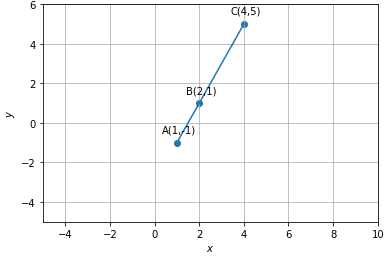
\includegraphics[scale=0.4]{sline.png} 
\caption{}
\end{figure}
\section{Code}
*Verify the above proofs in the following code.\\
\framebox{
\url{https://github.com/chandana531/FWC/tree/main/matrix/line}}	
\bibliographystyle{ieeetr}
\end{document}
